%GNUPLOT: LaTeX picture with Postscript
\begin{picture}(0,0)%
\includegraphics{Images/epslatex/Poincare_kappa_0.01.eps}%
\end{picture}%
\begingroup
\setlength{\unitlength}{0.0200bp}%
\begin{picture}(9900,6480)(0,0)%
\put(2200,5502){\makebox(0,0)[r]{\strut{} 0.4}}%
\put(2200,4646){\makebox(0,0)[r]{\strut{} 0.2}}%
\put(2200,3790){\makebox(0,0)[r]{\strut{} 0}}%
\put(2200,2934){\makebox(0,0)[r]{\strut{}-0.2}}%
\put(2200,2078){\makebox(0,0)[r]{\strut{}-0.4}}%
\put(9075,1100){\makebox(0,0){\strut{} 1.6}}%
\put(8250,1100){\makebox(0,0){\strut{} 1.4}}%
\put(7425,1100){\makebox(0,0){\strut{} 1.2}}%
\put(6600,1100){\makebox(0,0){\strut{} 1}}%
\put(5775,1100){\makebox(0,0){\strut{} 0.8}}%
\put(4950,1100){\makebox(0,0){\strut{} 0.6}}%
\put(4125,1100){\makebox(0,0){\strut{} 0.4}}%
\put(3300,1100){\makebox(0,0){\strut{} 0.2}}%
\put(2475,1100){\makebox(0,0){\strut{} 0}}%
\put(550,3790){\rotatebox{90}{\makebox(0,0){\strut{}$p_{\theta}$}}}%
\put(5775,275){\makebox(0,0){\strut{}$\theta$}}%
\end{picture}%
\endgroup
\endinput
